\subsection{Rayleigh-Taylor Instability}

This problem consists on the evolution of two layers of fluids initially at rest in the gravity field. The top layer is more dense than the one is placed at the bottom. Due to a little disturbance in the contact surface the more dense fluid goes down and the less dense fluid does the opposite. In the intermediate state a mixture is created, which is lately segregated. The final state reaches an stable equilibrium with the more dense fluid at the bottom layer and the less dense fluid at the top layer. The growth and evolution of the instability has been investigated among others by Tryggvason\cite{Tryggvason88} for inviscid incompressible flows, and by Guermond
\& Quartapelle\cite{Guermond00} for viscous flows.

The starting point is the problem documented by Guermond. The domain is $[-d/2,-2d]\times[d/2,2d]$. The initial position of the perturbed interface is $\eta(x) = 0.1d \cos(2\pi x/d)$. The heavy fluid is above and the density ratio is $3$, so that the Atwood
number is $0.5$ according to Tryggvason's definition $At = (\rho_{max}-\rho_{min})/(\rho_{max}+\rho_{min})$. Other physical parameters are selected to obtain $Re=\rho_{min}d^{\frac{3}{2}}g^{\frac{1}{2}}/\mu=1000$. Computational domain is discretized into $80000$ structured triangles ($\Delta x=0.01$) setting slip boundary conditions on each wall. Time step selected is $\Delta t=0.01[s]$, which allows to reach $CFL_{max} \approx 8$.

To compare with reference results, the time is made dimensionless by using $\widetilde{t} = t\sqrt{g\ At}$. Results on the vertical position of the tip of the falling and rising fluid (spike and bubble, respectively) are shown in Figure \ref{fg:rayleigh-rf}. It can be observed that current solution is in good agreement with the reference results.

\begin{figure}[H]
  \begin{center}
      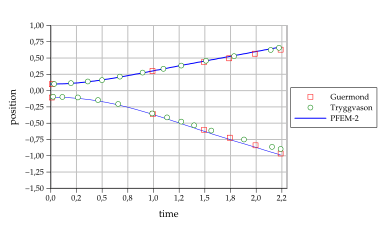
\includegraphics[width=\columnwidth]{images/rayleigh_1.pdf}
  \end{center}
  \caption{\label{fg:rayleigh-rf} Position of rising and falling bubbles versus time. Case with $Re=1000$.}
\end{figure}

On the other hand, the evolution of the instability is shown in Figure \ref{fg:rayleigh-screenshots} at dimensionless times $\widetilde{t}=0, 1, 1.5, 2$. Around $\widetilde{t}=1.5$ the heavy fluid begins to roll up into two counter-rotating vortices. Later, around $\widetilde{t} = 2$, these two vortices become unstable and a pair of secondary vortices appear at the tails of the roll-ups. These shapes of the fluid interface obtained with PFEM-2 are similar than those of the reference results.


\begin{figure}[htbp]
  \begin{center}
      \includegraphics[width=\columnwidth]{images/rayleigh_2_better.jpg}
  \end{center}
  \caption{\label{fg:rayleigh-screenshots} Rayleigh-Taylor instability evolution. Case with $Re=1000$. From left to right $\widetilde{t} =0.0$, $1.0$, $1.5$, $2.0$.}
\end{figure}

\subsubsection{Extending the time step}

In order to make emphasis in the capability of the method to manage large time-steps, the current case is also simulated with a large range of $\Delta t$ using the in-house implementation of PFEM and comparing with results obtained by the widely knows \OF suite. The problem setup and domain discretization is the same as presented above and the PFEM settings are not modified. 

In the case of \OF, the solver \texttt{interFoam} is chosen, which implements a Volume of Fluid (VoF) algorithm for multiphase flow\cite{Berberovic09}. It includes the multi-dimensional limiter for explicit solution (MULES) as a method of guaranteeing boundedness of scalar fields, in particular phase/mass-fractions (more information about MULES can be found in \cite{Marquez13}). Since \OF version 2.3, a new semi-implicit variant of MULES is introduced which combines operator splitting with application of the MULES limiter to an explicit correction rather than to the complete flux. This approach would maintain boundedness and stability at an arbitrarily large Courant number. In next simulation, the recommended schemes for the simulation have been used: \texttt{CrankNicolson} (second order, implicit) time integration, \texttt{Gauss linear} (second order, Gaussian integration with linear interpolation) discretization for the gradient, divergence and Laplacian operators (\texttt{corrected} with two \texttt{
nNonOrthogonalCorrectors} due to the triangular mesh, for the later ). Relevant VoF settings are: \texttt{nAlphaSubCycles} is set in order to keep the CFL of the sub-cycling around $0.5$, \texttt{cAlpha}$=0.25$ to give more stability through relaxing in some level the strong sharpness imposition, and \texttt{MULESCorr} is enabled to calculate the limiter in a semi-implicit way.

The set of figures in \ref{fg:rayleigh-comparison-dts} presents the comparison of the solutions with PFEM and \OF at a particular time ($\widehat{t}=2.25$) using several fixed time-steps (with the largest time-step a $CFL_{max}=15$ is reached). From captures, it can be shown that PFEM keeps approximately the same solution with each time-step, but interFoam can not solve with any accuracy using $\Delta t>0.001$ because the evolution of the mushroom-like interface differs form the reference results and this mistake is increased with large time-steps. Moreover, each simulation of interFoam diverges when $CFL_{mean}>0.5$ is reached (this happens at different times, depending on selected time-step). Another relevant feature to take into account is that the CPU times to solve a unique time-step is almost equal using both algorithms.

\begin{figure}[htbp]
  \begin{center}

      \includegraphics[width=.24\columnwidth]{images/rayleigh_foam_dts_A.jpg}
      \includegraphics[width=.24\columnwidth]{images/rayleigh_foam_dts_B.jpg}
      \includegraphics[width=.24\columnwidth]{images/rayleigh_foam_dts_C.jpg}
      \includegraphics[width=.24\columnwidth]{images/rayleigh_foam_dts_D.jpg}
      
      \includegraphics[width=.24\columnwidth]{images/rayleigh_pfem_dts_A.jpg}
      \includegraphics[width=.24\columnwidth]{images/rayleigh_pfem_dts_B.jpg}
      \includegraphics[width=.24\columnwidth]{images/rayleigh_pfem_dts_C.jpg}
      \includegraphics[width=.24\columnwidth]{images/rayleigh_pfem_dts_D.jpg}
      
  \end{center}
  \caption{\label{fg:rayleigh-comparison-dts} Rayleigh-Taylor instability capture for $\widetilde{t}=2.25$. Above PFEM simulations, below VoF+MULES simulation (InterFoam solver - OpenFoam suite). From left to right $\Delta t =0.001[s]$, $0.0025[s]$, $0.01[s]$, $0.025[s]$.}
\end{figure}
\afterpage{\clearpage}

